%------------------------------------------------------%
%------------------------------------------------------%
\section{Linear Programming}
%------------------------------------------------------%
%------------------------------------------------------%

%------------------------------------------------------%
\subsection{Examples}
Example 1: Consider the system of constraints \(\boldsymbol{A} \boldsymbol{x}=\boldsymbol{b}, \boldsymbol{x} \geq \boldsymbol{0}\) with

\begin{equation*}
	\boldsymbol{A}=\left[\begin{array}{llllll}
		1 & 4 & 7 & 1 & 0 & 0 \\
		2 & 5 & 8 & 0 & 1 & 0 \\
		3 & 6 & 9 & 0 & 0 & 1
	\end{array}\right], \boldsymbol{b}=\left[\begin{array}{l}
		12 \\
		15 \\
		18
	\end{array}\right]
\end{equation*}

Is \(\boldsymbol{x}=\left[\begin{array}{llllll}1 & 1 & 1 & 0 & 0 & 0\end{array}\right]^{\top}\) a basic feasible point?

\textbf{Short answer}:
and

Let \(\boldsymbol{x}=\left[\boldsymbol{x}_{\boldsymbol{B}}^{\top}, 0^{\top}\right]^{\top}\). Let \(\boldsymbol{A}=\left[\begin{array}{ll}\boldsymbol{B} & \boldsymbol{I}_{3}\end{array}\right]\), where \(\boldsymbol{I}_{3} \in \mathbb{R}^{3 \times 3}\) is the identity matrix

\begin{equation*}
	\boldsymbol{B}=\left[\begin{array}{lll}
		1 & 4 & 7 \\
		2 & 5 & 8 \\
		3 & 6 & 9
	\end{array}\right]
\end{equation*}

We call \(\boldsymbol{x}\) a basic solution to \(\boldsymbol{A} \boldsymbol{x}=\boldsymbol{b}\) with respect to the basis \(\boldsymbol{B}\). A vector \(\boldsymbol{x}\) satisfying \(\boldsymbol{A} \boldsymbol{x}=\boldsymbol{b}, \boldsymbol{x} \geq \boldsymbol{0}\), is said to be a feasible solution. A feasible solution that is also basic is called a basic feasible solution.

We first check if the solution is basic as follows:

Since \(\operatorname{rank}(\boldsymbol{B})=2<3\), the matrix \(\boldsymbol{B}\) is singular. Therefore, \(\boldsymbol{B}\) cannot be a basis, and we do not have a basic solution corresponding to \(\boldsymbol{B}\).

We then check if the solution is feasible as follows:

\begin{equation*}
	\boldsymbol{A} \boldsymbol{x}=\left[\begin{array}{llllll}
		1 & 4 & 7 & 1 & 0 & 0 \\
		2 & 5 & 8 & 0 & 1 & 0 \\
		3 & 6 & 9 & 0 & 0 & 1
	\end{array}\right]\left[\begin{array}{l}
		1 \\
		1 \\
		1 \\
		0 \\
		0 \\
		0
	\end{array}\right]=\left[\begin{array}{l}
		12 \\
		15 \\
		18
	\end{array}\right]=\boldsymbol{b} .
\end{equation*}

And \(\boldsymbol{x} \geq \boldsymbol{0}\). So, the solution \(\boldsymbol{x}\) is a feasible solution to \(\boldsymbol{A} \boldsymbol{x}=\boldsymbol{b}\).

Therefore, \(\boldsymbol{x}\) is not a basic feasible point. Indeed, \(\boldsymbol{x}\) is feasible but non-basic.

\medskip
\noindent
Example 2: Suppose that a linear program originally included a free variable \(x_{i}\) where there were no upper and lower bounds on its values. This can be converted into a pair of variables \(x_{i}^{+}\)and \(x_{i}^{-}\)such that \(x_{i}^{+}, x_{i}^{-} \geq 0\) and \(x_{i}\) is replaced with the difference \(x_{i}^{+}-x_{i}^{-}\). Prove that a basic feasible point can have only one of \(x_{i}^{+}\)or \(x_{i}^{-}\)different from zero.

\textbf{Short answer}:

Consider the optimization problem

\[
	\begin{array}{rl}
		\operatorname{mininize} &  c_{1}\left|x_{1}\right|+c_{2}\left|x_{2}\right|+\cdots+c_{n}\left|x_{n}\right| \\
		& \\
		\text { subject to} & \boldsymbol{A} \boldsymbol{x}=\boldsymbol{b} .
	\end{array}
\]

Let \(x_{i}^{+}, x_{i}^{-} \geq 0\) be such that \(\left|x_{i}\right|=x_{i}^{+}+x_{i}^{-}, x_{i}=x_{i}^{+}-x_{i}^{-}\). Substituting into the original problem, we have

\[
	\begin{array}{rl}
		\operatorname{mininize} & c_{1}\left(x_{1}^{+}+x_{1}^{-}\right)+c_{2}\left(x_{2}^{+}+x_{2}^{-}\right)+\cdots+c_{n}\left(x_{n}^{+}+x_{n}^{-}\right) \\
		\text {subject to} & \boldsymbol{A} \left(\boldsymbol{x}^{+}-\boldsymbol{x}^{-}\right)=\boldsymbol{b} \\
		& \boldsymbol{x}^{+}, \boldsymbol{x}^{-} \geq \boldsymbol{0}
	\end{array}
\]

where \(\boldsymbol{x}^{+}=\left[x_{1}^{+}, \ldots, x_{n}^{+}\right]^{\top}\) and \(\boldsymbol{x}^{-}=\left[x_{1}^{-}, \ldots, x_{n}^{-}\right]^{\top}\). Rewriting, we get

\[
	\begin{array}{rl}
		\operatorname{mininize} & {\left[\boldsymbol{c}^{\top}, \boldsymbol{c}^{\top}\right] \boldsymbol{z} } \\
		& \\
		\text { subject to} & {[\boldsymbol{A},-\boldsymbol{A}] \boldsymbol{z}=\boldsymbol{b} } \\
		& \boldsymbol{z} \geq \boldsymbol{0}.
	\end{array}
\]

which is an equivalent linear programming problem in standard form.

Note that although the variables \(x_{i}^{+}\)and \(x_{i}^{-}\)in the solution are required to satisfy \(x_{i}^{+} x_{i}^{-}=0\), we do not need to explicitly include this in the constraint because any optimal solution to the above transformed problem automatically satisfies the condition \(x_{i}^{+} x_{i}^{-}=0\). To see this, suppose we have an optimal solution with both \(x_{i}^{+}\)and \(x_{i}^{-}>0\). In this case, note that \(c_{i}>0\). Then by subtracting \(\min \left(x_{i}^{+}, x_{i}^{-}\right)\)from \(x_{i}^{+}\)and \(x_{i}^{-}\), we have a new feasible point with lower objective function value, contradicting the optimality assumption.

We now prove that a basic feasible point can have only one of \(x_{i}^{+}\)or \(x_{i}{ }^{-}\) different from zero in another angle as follows.

The columns in the constraint matrix \(A\) corresponding to \(x_{i}^{+}\)and \(x_{i}^{-}\)are linearly dependent. Hence they cannot both enter a basis at the same time. This means that only one variable, \(x_{i}^{+}\)or \(x_{i}^{-}\), can assume a non-negative value; the non-basic variable is necessarily zero.

\medskip
\noindent
Example 3: Illustrate the behavior of the simplex method on the LP

\[
	\begin{array}{rl}
		\operatorname{mininize} & -x_{1}-3 x_{2} \\
		& \\
		\text { subject to} & -2 x_{1}+x_{2} \leq 2 \\
		& -x_{1}+2 x_{2} \leq 7 \\
		& x \geq 0.
	\end{array}
\]

starting at \(\left[\begin{array}{ll}0 & 0\end{array}\right]^{\top}\) after converting the problem to the standard form.

\textbf{Short answer}:

We first convert the LP into the standard form

\[
	\begin{array}{rl}
		\operatorname{mininize} & -x_{1}-3 x_{2} \\
		& \\
		\text { subject to} & -2 x_{1}+x_{2}+x_{3}=2 \\
		& -x_{1}+2 x_{2}+x_{4}=7 \\
		& x_{1}, x_{2}, x_{3}, x_{4} \geq 0 .
	\end{array}
\]


The problem has no solution because it is unbounded, We explain it as follows. From the inequality constraints, we have

\begin{equation*}
	\begin{aligned}
		& x_{2} \leq 2 x_{1}+2 \\
		& x_{2} \leq x_{1}+\frac{7}{2} \\
		& x_{1}, x_{2} \geq 0
	\end{aligned}
\end{equation*}

Clearly, \(x_{1}\) can be infinitely large. Since \(x_{2}\) is upper bounded by \(x_{1}\), we can also have \(x_{2}\) to be infinitely large. Therefore, \(f=x_{1}+3 x_{2}\) can be infinitely large, there is no maximize solution for this case. If we use the simplex method, we will get the follows. As it is shown in the below figure, after 3 iterations, the BFS goes back to \(\boldsymbol{x}^{*}=\left[\begin{array}{llll}0 & 0 & 2 & 7\end{array}\right]^{\top}\) again, the algorithm is circling, it never ends, it can not solve this problem as expected.

\begin{center}
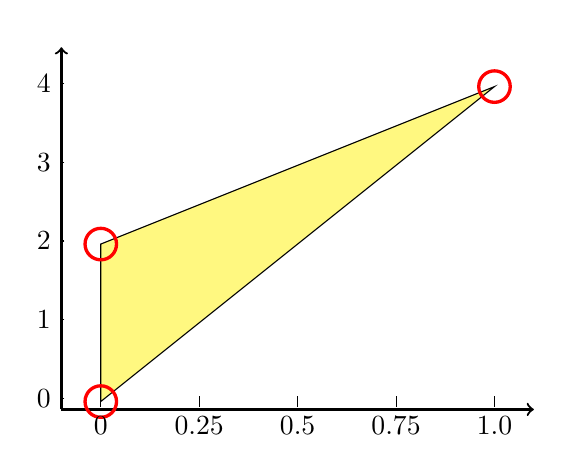
\begin{tikzpicture}
	\begin{scope}[xscale=5, yscale=1]
		% Draw triangle 
		\filldraw[fill=yellow!50] (0,0) -- (0,2) -- (1,4) -- cycle;
		
		% Draw axes
		\draw[thick,->] (-0.1,-0.1) -- (1.1,-0.1) node[right] {};
		\draw[thick,->] (-0.1,-0.1) -- (-0.1,4.5) node[above] {};
	\end{scope}
	
	\foreach \point/\xscale/\yscale in {(0,0)/5/1, (0,2)/5/1, (5,4)/5/1}{
		\draw[red, very thick] \point circle[radius=2mm] node[transform shape, scale=1/\xscale] {};
	}
	% Draw ticks on x-axis and y-axis
	\foreach \x in {0,0.25, 0.5,0.75,1.0} % Adjust or add values for ticks as needed
	\draw[xscale=5] (\x,2pt) -- (\x,-2pt) node[below] {\(\x\)};
	
	\foreach \y in {0,1,...,4} % Adjust or add values for ticks as needed
	\draw (-0.5pt,\y, -0.1) -- (-0.55pt,\y, -0.1) node[left] {\(\y\)};
	
\end{tikzpicture}
\end{center}


\medskip
\noindent
Example 4: Consider the following linear programming problem

\[
	\begin{array}{rl}
		\operatorname{mininize} & -\frac{3}{4} x_{4}+20 x_{5}-\frac{1}{2} x_{6}+6 x_{7} \vspace{2mm}\\
		\text { subject to} & x_{1}+\frac{1}{4} x_{4}-8 x_{5}-x_{6}+9 x_{7}=0 \vspace{2mm}\\
		& x_{2}+\frac{1}{2} x_{4}-12 x_{5}-\frac{1}{2} x_{6}+3 x_{7}=0 \vspace{2mm}\\
		& x_{3}+x_{6}=1 \vspace{2mm}\\
		& x_{1}, \ldots, x_{7} \geq 0 .
	\end{array}
\]

(1) Apply the simplex algorithm to the problem using the rule that \(q\) is the index corresponding to the most negative \(r_{q}\). (As usual, if more than one index \(i\) minimizes \(y_{i 0} / y_{i q}\), let \(p\) be the smallest such index.) Start with \(x_{1}, x_{2}\), and \(x_{3}\) as initial basic variables. Notice that cycling occurs.

(2) Repeat part (1) using Bland's rule for choosing \(q\) and \(p\) :

\begin{equation*}
	\begin{aligned}
		& q=\min \left\{i: r_{i}<0\right\}, \\
		& p=\min \left\{j: y_{j 0} / y_{j q}=\min _{i}\left\{y_{i 0} / y_{i q}: y_{i q}>0\right\}\right\} .
	\end{aligned}
\end{equation*}

\textbf{Short answer}:
(1) We form the tableau for the problem

\begin{equation*}
	\begin{array}{cccccccc}
		1 & 0 & 0 & 1 / 4 & -8 & -1 & 9 & 0 \\
		0 & 1 & 0 & 1 / 2 & -12 & -1 / 2 & 3 & 0 \\
		0 & 0 & 1 & 0 & 0 & 1 & 0 & 1 \\
		0 & 0 & 0 & -3 / 4 & 20 & -1 / 2 & 6 & 0
	\end{array}
\end{equation*}

The above tableau is already in canonical form, and therefore we can process with simplex procedure.

We first pivot about \((1,4)\) th element, to get

\begin{equation*}
	\begin{array}{cccccccc}
		4 & 0 & 0 & 1 & -32 & -4 & 36 & 0 \\
		-2 & 1 & 0 & 0 & 4 & 3 / 2 & -15 & 0 \\
		0 & 0 & 1 & 0 & 0 & 1 & 0 & 1 \\
		3 & 0 & 0 & 0 & -4 & -7 / 2 & 33 & 0
	\end{array}
\end{equation*}

Pivoting about \((2,5)\) th element, we get

\begin{equation*}
	\begin{array}{cccccccc}
		-12 & 8 & 0 & 1 & 0 & 8 & -84 & 0 \\
		-1 / 2 & 1 / 4 & 0 & 0 & 1 & 3 / 8 & -15 / 4 & 0 \\
		0 & 0 & 1 & 0 & 0 & 1 & 0 & 1 \\
		1 & 1 & 0 & 0 & 0 & -2 & 18 & 0
	\end{array}
\end{equation*}

Pivoting about \((1,6)\) th element, we get

\begin{equation*}
	\begin{array}{cccccccc}
		-3 / 2 & 1 & 0 & 1 / 8 & 0 & 1 & -21 / 2 & 0 \\
		1 / 16 & -1 / 8 & 0 & -3 / 64 & 1 & 0 & 3 / 16 & 0 \\
		3 / 2 & -1 & 1 & -1 / 8 & 0 & 0 & 21 / 2 & 1 \\
		-2 & 3 & 0 & 1 / 4 & 0 & 0 & -3 & 0
	\end{array}
\end{equation*}

Pivoting about \((2,7)\) th element, we get

\begin{equation*}
	\begin{array}{cccccccc}
		2 & -6 & 0 & -5 / 2 & 56 & 1 & 0 & 0 \\
		1 / 3 & -2 / 3 & 0 & -1 / 4 & 16 / 3 & 0 & 1 & 0 \\
		-2 & 6 & 1 & 5 / 2 & -56 & 0 & 0 & 1 \\
		-1 & 1 & 0 & -1 / 2 & 16 & 0 & 0 & 0
	\end{array}
\end{equation*}

Pivoting about \((1,1)\) th element, we get

\begin{equation*}
	\begin{array}{cccccccc}
		1 & -3 & 0 & -5 / 4 & 28 & 1 / 2 & 0 & 0 \\
		0 & 1 / 3 & 0 & 1 / 6 & -4 & -1 / 6 & 1 & 0 \\
		0 & 0 & 1 & 0 & 0 & 1 & 0 & 1 \\
		0 & -2 & 0 & -7 / 4 & 44 & 1 / 2 & 0 & 0
	\end{array}
\end{equation*}

Pivoting about \((2,2)\) th element, we get

\begin{equation*}
	\begin{array}{cccccccc}
		1 & 0 & 0 & 1 / 4 & -8 & -1 & 9 & 0 \\
		0 & 1 & 0 & 1 / 2 & -12 & -1 / 2 & 3 & 0 \\
		0 & 0 & 1 & 0 & 0 & 1 & 0 & 1 \\
		0 & 0 & 0 & -3 / 4 & 20 & -1 / 2 & 6 & 0
	\end{array}
\end{equation*}

which is identical to initial tableau. Therefore, cycling occurs.

(2) We start with initial tableau of part (1), and pivot about the \((1,4)\) th element to obtain

\begin{equation*}
	\begin{array}{cccccccc}
		4 & 0 & 0 & 1 & -32 & -4 & 36 & 0 \\
		-2 & 1 & 0 & 0 & 4 & 3 / 2 & -15 & 0 \\
		0 & 0 & 1 & 0 & 0 & 1 & 0 & 1 \\
		3 & 0 & 0 & 0 & -4 & -7 / 2 & 33 & 0
	\end{array}
\end{equation*}

Pivoting about \((2,5)\) th element, we get

\begin{equation*}
	\begin{array}{cccccccc}
		-12 & 8 & 0 & 1 & 0 & 8 & -84 & 0 \\
		-1 / 2 & 1 / 4 & 0 & 0 & 1 & 3 / 8 & -15 / 4 & 0 \\
		0 & 0 & 1 & 0 & 0 & 1 & 0 & 1 \\
		1 & 1 & 0 & 0 & 0 & -2 & 18 & 0
	\end{array}
\end{equation*}

Pivoting about \((1,6)\) th element, we get

\begin{equation*}
	\begin{array}{cccccccc}
		-3 / 2 & 1 & 0 & 1 / 8 & 0 & 1 & -21 / 2 & 0 \\
		1 / 16 & -1 / 8 & 0 & -3 / 64 & 1 & 0 & 3 / 16 & 0 \\
		3 / 2 & -1 & 1 & -1 / 8 & 0 & 0 & 21 / 2 & 1
	\end{array}
\end{equation*}

Pivoting about \((2,1)\) th element, we get

\begin{equation*}
	\begin{array}{cccccccc}
		0 & -2 & 0 & -1 & 24 & 1 & -6 & 0 \\
		1 & -2 & 0 & -3 / 4 & 16 & 0 & 3 & 0 \\
		0 & 2 & 1 & 1 & -24 & 0 & 6 & 1 \\
		0 & -1 & 0 & -5 / 4 & 32 & 0 & 3 & 0
	\end{array}
\end{equation*}

Pivoting about \((3,2)\) th element, we get

\begin{equation*}
	\begin{array}{cccccccc}
		0 & 0 & 1 & 0 & 0 & 1 & 0 & 1 \\
		1 & 0 & 1 & 1 / 4 & -8 & 0 & 9 & 1 \\
		0 & 1 & 1 / 2 & 1 / 2 & -12 & 0 & 3 & 1 / 2 \\
		0 & 0 & 1 / 2 & -3 / 4 & 20 & 0 & 6 & 1 / 2
	\end{array}
\end{equation*}

Pivoting about \((3,2)\) th element, we get

\begin{equation*}
	\begin{array}{cccccccc}
		0 & 0 & 1 & 0 & 0 & 1 & 0 & 1 \\
		1 & -1 / 2 & 3 / 4 & 0 & -2 & 0 & 15 / 2 & 3 / 4 \\
		0 & 2 & 1 & 1 & -24 & 0 & 6 & 1 \\
		0 & 3 / 2 & 5 / 4 & 0 & 2 & 0 & 21 / 2 & 5 / 4
	\end{array}
\end{equation*}

The reduced cost coefficient are all nonnegative. Hence, the optimal solution to the problem is \(\left[\begin{array}{lllllll}3 / 4 & 0 & 0 & 1 & 0 & 1 & 0\end{array}\right]^{\top}\). The corresponding optimal cost is \(-5 / 4\).
